%%This is a very basic article template.
%%There is just one section and two subsections.
\documentclass{article}
\usepackage[latin1]{inputenc} %coding of writteninput %latin1 allows for Umlaute
\usepackage[T1]{fontenc}%vectorized fonts (cm-super package)
\usepackage[german]{babel}%some specifics of the german language
\usepackage{amsfonts, amsmath, amsthm, amssymb, mathabx, paralist}
\setlength{\parindent}{0em} 
\usepackage{listings}
\usepackage{pdfpages}
 \lstset{language=Matlab,%
    %basicstyle=\color{red},
    breaklines=true,%
    morekeywords={matlab2tikz},
    keywordstyle=\color{blue},%
    morekeywords=[2]{1}, keywordstyle=[2]{\color{black}},
    identifierstyle=\color{black},%
    stringstyle=\color{mylilas},
    commentstyle=\color{mygreen},%
    showstringspaces=false,%without this there will be a symbol in the places where there is a space
    numbers=left,%
    numberstyle={\tiny \color{black}},% size of the numbers
    numbersep=9pt, % this defines how far the numbers are from the text
    emph=[1]{for,end,break},emphstyle=[1]\color{red}, %some words to emphasise
    %emph=[2]{word1,word2}, emphstyle=[2]{style},    
}

 %Decisiontree
 \usepackage{tikz,forest}
 \usepackage{tikz}
\usetikzlibrary{arrows,shapes,snakes,automata,backgrounds,petri}
\usetikzlibrary{arrows.meta}
  
\usepackage{graphicx} 

\usepackage{verbatim}%f�r txt datei

\usepackage{color} %red, green, blue, yellow, cyan, magenta, black, white
\definecolor{mygreen}{RGB}{28,172,0} % color values Red, Green, Blue
\definecolor{mylilas}{RGB}{170,55,241}

\title{Homework 1}
\author{ Miriam Wagner\\373045}
\begin{document}
\maketitle
\section*{Question 1}
I used for solving this exercise Matlab. My code you can see here:
\lstinputlisting{clustering.m}

The functions used I does not write down them here. 'distance' calculates the
euclidian distance and centroid sums up all vectors and divides by the number of
vectors.

My clustering algorithm now calculates for every Datavector the distances to
every centroid and then checks which centroid is closed. The vector is add to
the cluster. When all datavectors are put in a cluster the new cluster centroids
are calculated. 

My abort criterion is the change between the centroids. If they still change I
will apply the algorithms again. Because of the computer accuracy I do not use
0, but $10^{-15}$.
% Table generated by Excel2LaTeX from sheet 'Blad1'
\begin{table}[h]
  \centering
  \caption{Distances first round}
    \begin{tabular}{rrr}
    \multicolumn{1}{l}{distance\_to\_cluster\_1} & \multicolumn{1}{l}{distance\_to\_cluster\_2} & \multicolumn{1}{l}{distance\_to\_cluster\_3} \\
    0     & 4     & 20 \\
    68    & 64    & 48 \\
    3     & 7     & 23 \\
    19    & 15    & 1 \\
    20    & 16    & 0 \\
    1     & 3     & 19 \\
    39    & 35    & 19 \\
    40    & 36    & 20 \\
    4     & 0     & 16 \\
    82    & 78    & 62 \\
    19    & 15    & 1 \\
    5     & 1     & 15 \\
    16    & 12    & 4 \\
    0     & 4     & 20 \\
    35    & 31    & 15 \\
    3     & 7     & 23 \\
    46    & 42    & 26 \\
    3     & 7     & 23 \\
    6     & 2     & 14 \\
    9     & 5     & 11 \\
    \end{tabular}%
  \label{tab:dist1}%
\end{table}%
The algorithm finds after two rounds already good enough clusters.
The distances in the first round are to see in \ref{tab:dist1}

% Table generated by Excel2LaTeX from sheet 'Blad1'
\begin{table}[ht]
  \centering
  \caption{centroid}
    \begin{tabular}{rrr}
    \multicolumn{1}{l}{centroid\_1} & \multicolumn{1}{l}{centroid\_2} & \multicolumn{1}{l}{centroid\_3} \\
    7000  & 13000 & 15000 \\
    0,29309 & 0,515625 & 28,43964 \\
    6     & 10    & 74 \\
    \end{tabular}%
  \label{tab:centr1}%
\end{table}%
The new centroids are in \ref{tab:centr1}

% Table generated by Excel2LaTeX from sheet 'Sheet2'
\begin{table}[ht]
  \centering
  \caption{Distances second round}
    \begin{tabular}{rrr}
    \multicolumn{1}{l}{distance\_to\_cluster\_1} & \multicolumn{1}{l}{distance\_to\_cluster\_2} & \multicolumn{1}{l}{distance\_to\_cluster\_3} \\
    0     & 4     & 68 \\
    68    & 64    & 0 \\
    3     & 7     & 71 \\
    19    & 15    & 49 \\
    20    & 16    & 48 \\
    1     & 3     & 67 \\
    39    & 35    & 29 \\
    40    & 36    & 28 \\
    4     & 0     & 64 \\
    82    & 78    & 14 \\
    19    & 15    & 49 \\
    5     & 1     & 63 \\
    16    & 12    & 52 \\
    0     & 4     & 68 \\
    35    & 31    & 33 \\
    3     & 7     & 71 \\
    46    & 42    & 22 \\
    3     & 7     & 71 \\
    6     & 2     & 62 \\
    9     & 5     & 59 \\
          &       &  \\
    \end{tabular}%
  \label{tab:dist2}%
\end{table}%
And the centroids in \ref{tab:cent2}
% Table generated by Excel2LaTeX from sheet 'Sheet2'
\begin{table}[ht]
  \centering
  \caption{centroids second round}
    \begin{tabular}{rrr}
    \multicolumn{1}{l}{centroid\_1} & \multicolumn{1}{l}{centroid\_2} & \multicolumn{1}{l}{centroid\_3} \\
    7000  & 13000 & 15000 \\
    0,29309 & 0,515625 & 28,43964 \\
    6     & 10    & 74 \\
          &       &  \\
    \end{tabular}%
  \label{tab:cent2}%
\end{table}%
The next round the distances are in \ref{tab:dist2}


% Table generated by Excel2LaTeX from sheet 'Blad1'
\begin{table}[ht]
  \centering
  \caption{Cluster 1}
    \begin{tabular}{rrrr}
    \multicolumn{1}{l}{amount\_req} & \multicolumn{1}{l}{case\_duration} & \multicolumn{1}{l}{total\_activities} &  \\
    7000  & 0,29309 & 6     &  \\
    23112 & 0,000532 & 3     &  \\
    2500  & 0,021134 & 7     &  \\
    6500  & 0,002049 & 6     &  \\
    10000 & 0,000799 & 3     &  \\
    8500  & 0,000486 & 3     &  \\
    7000  & 0,29309 & 6     &  \\
    23112 & 0,000532 & 3     &  \\
    2500  & 0,021134 & 7     &  \\
    6500  & 0,002049 & 6     &  \\
    10000 & 0,000799 & 3     &  \\
    8500  & 0,000486 & 3     &  \\
    \end{tabular}%
  \label{tab:clust1}%
\end{table}%
Cluster1 contains \ref{tab:clust1}

% Table generated by Excel2LaTeX from sheet 'Blad1'
\begin{table}[ht]
  \centering
    \caption{Cluster 2}
    \begin{tabular}{rrr}
    \multicolumn{1}{l}{amount\_req} & \multicolumn{1}{l}{case\_duration} & \multicolumn{1}{l}{total\_activities} \\
    13000 & 0,515625 & 10 \\
    7500  & 0,489861 & 11 \\
    17000 & 0,01375 & 12 \\
    3000  & 6,955382 & 15 \\
    6000  & 0,048206 & 25 \\
    10000 & 12,95023 & 26 \\
    13000 & 0,515625 & 10 \\
    5000  & 7,612419 & 25 \\
    7500  & 0,489861 & 11 \\
    6000  & 6,503808 & 22 \\
    25000 & 21,14506 & 41 \\
    17000 & 0,01375 & 12 \\
    3000  & 6,955382 & 15 \\
          &       &  \\
          &       &  \\
    \end{tabular}%
  \label{tab:clust2}%
\end{table}%
Cluster 2 contains as in \ref{tab:clust2}


% Table generated by Excel2LaTeX from sheet 'Blad1'
\begin{table}[ht]
  \centering
  \caption{cluster 3}
    \begin{tabular}{rrr}
    \multicolumn{1}{l}{amount\_req} & \multicolumn{1}{l}{case\_duration} & \multicolumn{1}{l}{total\_activities} \\
    15000 & 28,43964 & 74 \\
    6000  & 0,048206 & 25 \\
    10000 & 12,95023 & 26 \\
    19000 & 19,78213 & 45 \\
    5000  & 29,51885 & 46 \\
    35000 & 19,74352 & 88 \\
    5000  & 7,612419 & 25 \\
    6000  & 6,503808 & 22 \\
    25000 & 21,14506 & 41 \\
    7800  & 19,1099 & 52 \\
    15000 & 28,43964 & 74 \\
    19000 & 19,78213 & 45 \\
    5000  & 29,51885 & 46 \\
    35000 & 19,74352 & 88 \\
    7800  & 19,1099 & 52 \\
          &       &  \\
    \end{tabular}%
  \label{tab:clust3}%
\end{table}%

Cluster 3 in \ref{tab:clust3}

\clearpage
\section*{Question 2}
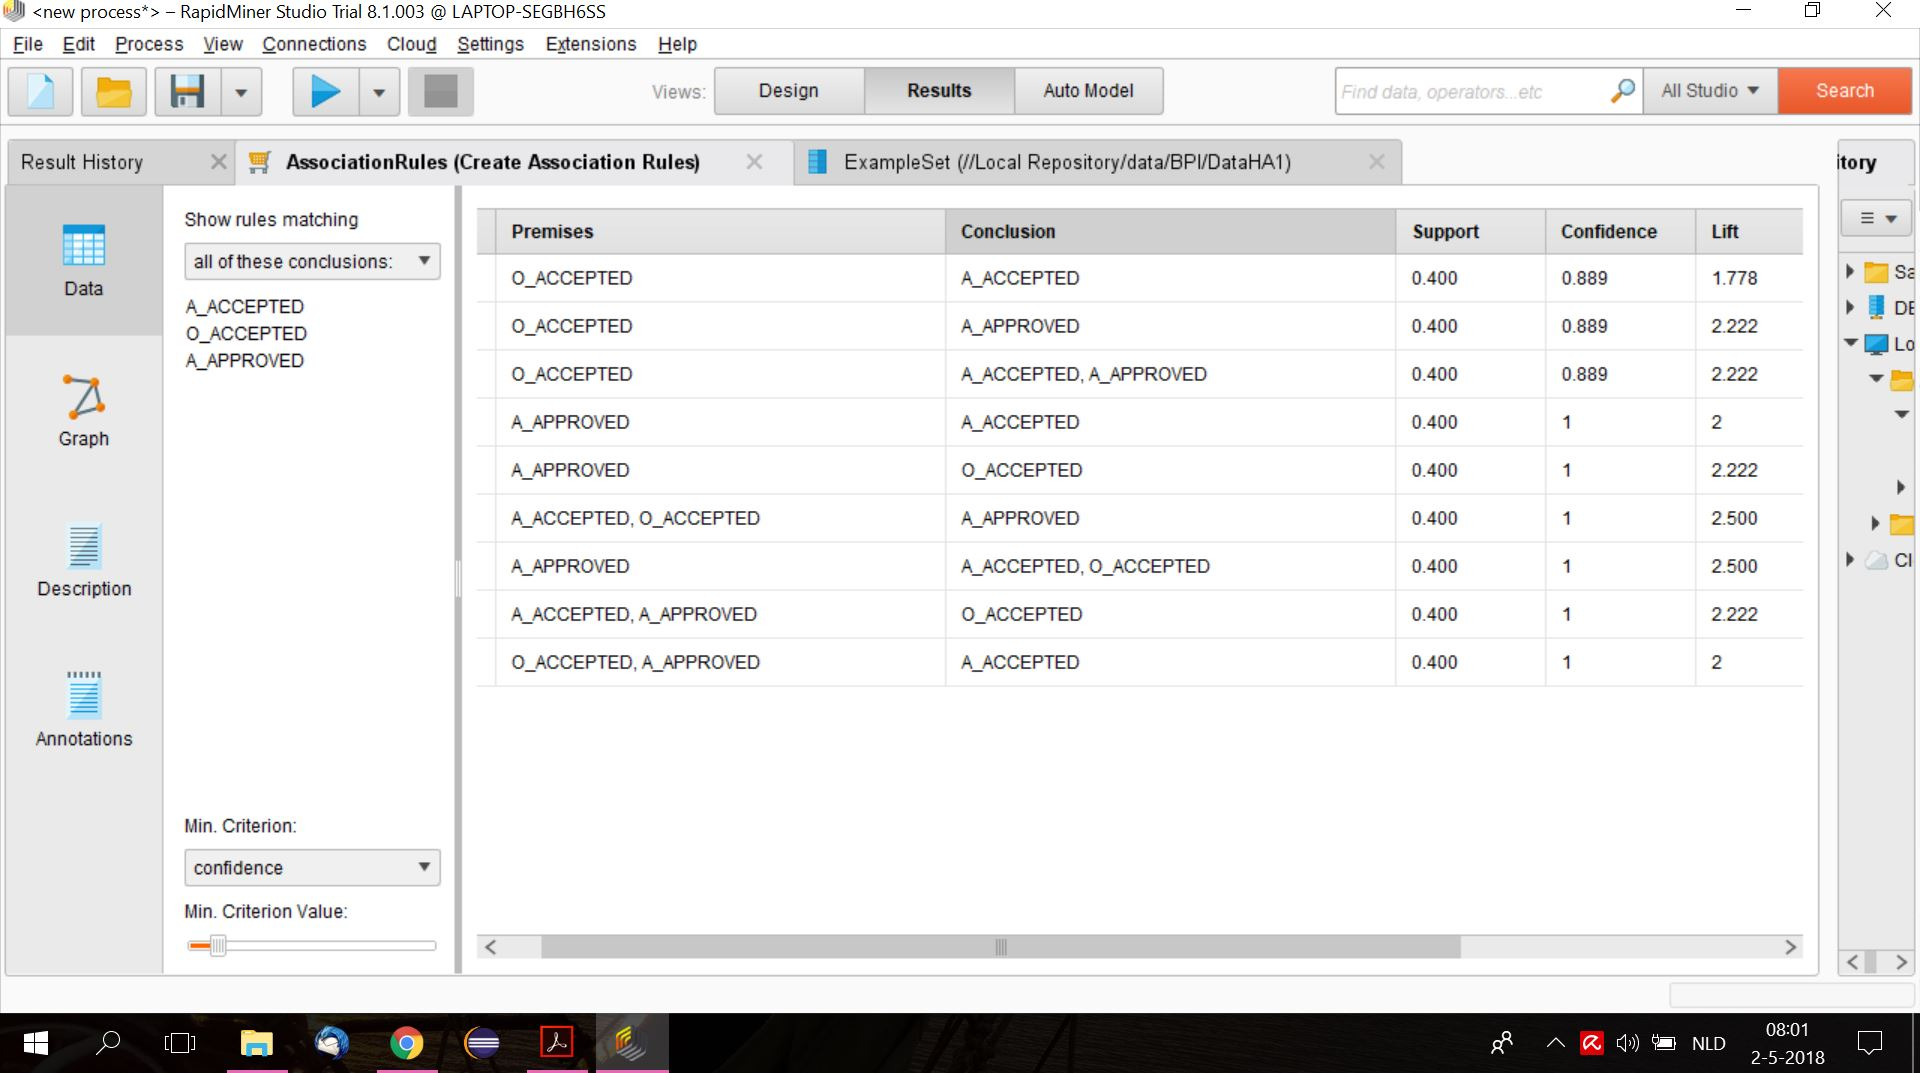
\includegraphics[width=1.8\textwidth, angle =90 ]{Question2Rapid.jpg}

I would pick the rule \{A\_ACCEPTED, O\_ACCEPTED\} $\Rightarrow$	\{A\_APPROVED\}
and \{A\_APPROVED\} $\Rightarrow$	\{A\_ACCEPTED, O\_ACCEPTED\}, because they
have the highest lift, confidence and support. When you have a closer look you
will see that the sets are probably logical equivalent. Always pick the rule
with the best lift, confidence and support.

\section*{Question 3}

The found decision tree is 

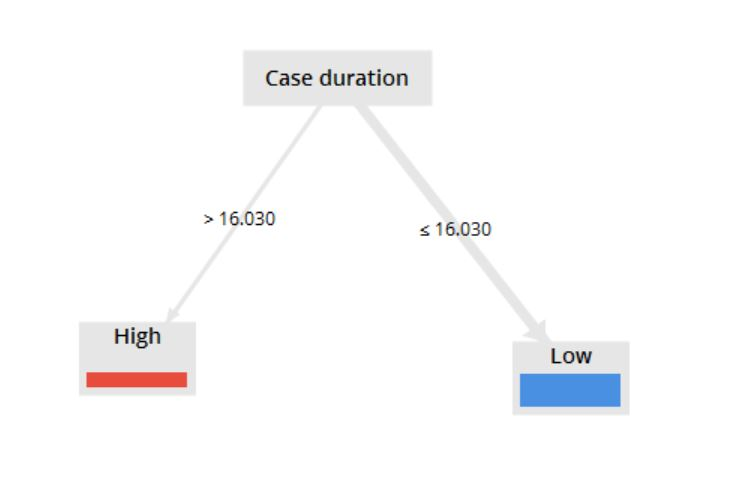
\includegraphics[width=0.8\textwidth]{Question3Deci.jpg}

If you check the Confusionmatrix

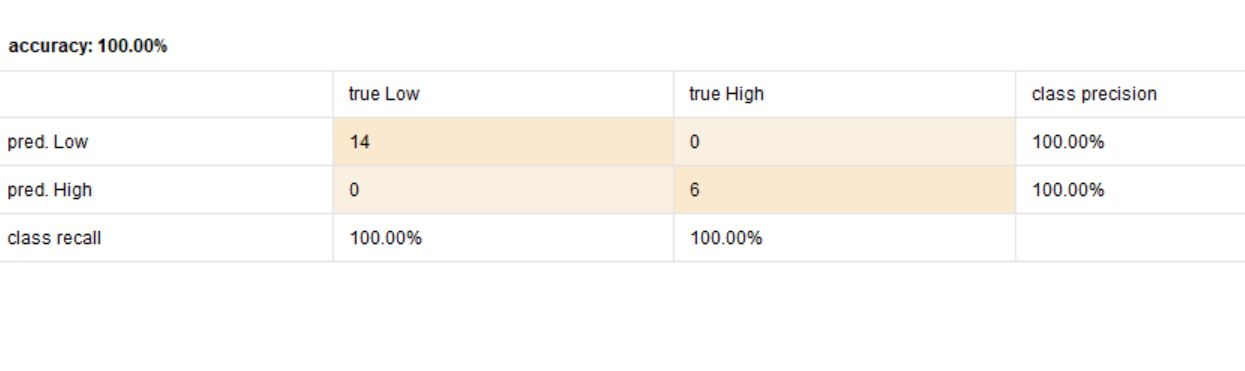
\includegraphics[width=0.8\textwidth]{Question3Confusion.jpg}

you see, that this decision tree classifys the data perfectly. So you can
predict by just knowing the case duration the total activities. If the case
duration is higher, than also the total activities are high. This seems to be
logical, if you have to do a lot this takes most of the times longer and
otherwise around, if you do not need long you mostly did not do a lot of
different things in the time.

\section*{Question 4}
\subsection*{1.}
\begin{equation*}
L1= [\langle a,b,e,f\rangle ,\langle a,b,e,c,d,b,f\rangle ,\langle a,b,c,e,d,b
,f\rangle ,\langle a,b,c,d,e,b,f\rangle ,\langle a,e,b,c,d,b,f\rangle ]
\end{equation*}
The $\alpha-$Algorithm gives the following:

\begin{align*}
T_L &= \{ a,b,c,d,e,f\}\\
T_I &= \{a\}\\
T_O &= \{f\}
\end{align*}
\begin{tabular}{c | c c c c c c}
	&a 	  &b 			 &c 			&d 	  			&e 			   &f\\
	\hline
a	&$\#$ &$\rightarrow$ &$\#$ 			&$\#$ 			&$\rightarrow$ &$\#$\\
b	&$\#$ &$\#$			 &$\rightarrow$ &$\#$ 			&$||$ 		   &$\rightarrow$\\
c	&$\#$ &$\#$			 &$\#$			&$\rightarrow$  &$||$ 		   &$\#$\\
d	&$\#$ &$\rightarrow$ &$\#$			&$\#$			&$||$ 		   &$\#$\\
e	&$\#$ &$||$ 		 &$||$			&$||$  			&$\#$		   &$\rightarrow$\\
f	&$\#$ &$\leftarrow$	 &$\#$			&$\#$			&$\#$		   &$\leftarrow$\\
\end{tabular}

\begin{align*}
X_L &= \{ (\{a\},\{b\})
,(\{a\},\{e\}),(\{b\},\{c\}),(\{b\},\{f\}),(\{c\},\{d\}),(\{b\},\{c,f\}),(\{d\},\{b\}),(\{e\},\{f\}),(\{a,d\},\{b\})\}\\
Y_L &= \{(\{a\},\{e\}),(\{b\},\{c,f\}),(\{b\},\{f\}),(\{c\},\{d\}),(\{e\},\{f\}),(\{a,d\},\{b\})\}\\
\end{align*}

\begin{tikzpicture}[node distance=1.3cm,>=stealth',bend angle=45,auto]

  \tikzstyle{place}=[circle,thick,draw=blue!75,fill=blue!20,minimum size=6mm]
  \tikzstyle{transition}=[rectangle,thick,draw=black!75,
  			  fill=black!20,minimum size=4mm]

  \tikzstyle{every label}=[red]

  \begin{scope}
    % First net
    \node [place,tokens=1] (start)                {};
    \node [transition] (a) [right of=start]       {a}
    	edge [pre] (start);
    \node [place] (toe)  [above right of=a]	  	  {}
    	edge [pre] (a);
    \node [place] (tob) [right of=a]        {}
    	edge [pre] (a);
    \node [transition] (e) [right of=toe]         {e}
    	edge [pre] (toe);
	\node [transition] (b) [right of=tob]         {b}
		edge [pre] (tob);
    \node [place] (etof) [right of=e] {}
    	edge [pre] (e);
    \node [place] (btof) [right of=b] {}
    	edge [pre] (b);
    \node [transition] (f) [right of=etof] {f}
    	edge [pre] (btof)
    	edge [pre] (etof);
    \node [place] (end) [right of=f] {}
    	edge [pre] (f);
    \node [place] (btoc) [below right of=b] {}
    	edge [pre] (b);
    \node [transition] (c) [below right of=btoc] {c}
    	edge [pre] (btoc);
    \node [place] (ctod) [below of=b] {}
    	edge [pre] (c);
    \node [transition] (d) [below of=a] {d}
    	edge [pre] (ctod)
    	edge [post] (tob);
  \end{scope}
\end{tikzpicture}
\end{document}
